\documentclass[11pt,preprint, authoryear]{elsarticle}

\usepackage{lmodern}
%%%% My spacing
\usepackage{setspace}
\setstretch{1.2}
\DeclareMathSizes{12}{14}{10}{10}

% Wrap around which gives all figures included the [H] command, or places it "here". This can be tedious to code in Rmarkdown.
\usepackage{float}
\let\origfigure\figure
\let\endorigfigure\endfigure
\renewenvironment{figure}[1][2] {
    \expandafter\origfigure\expandafter[H]
} {
    \endorigfigure
}

\let\origtable\table
\let\endorigtable\endtable
\renewenvironment{table}[1][2] {
    \expandafter\origtable\expandafter[H]
} {
    \endorigtable
}


\usepackage{ifxetex,ifluatex}
\usepackage{fixltx2e} % provides \textsubscript
\ifnum 0\ifxetex 1\fi\ifluatex 1\fi=0 % if pdftex
  \usepackage[T1]{fontenc}
  \usepackage[utf8]{inputenc}
\else % if luatex or xelatex
  \ifxetex
    \usepackage{mathspec}
    \usepackage{xltxtra,xunicode}
  \else
    \usepackage{fontspec}
  \fi
  \defaultfontfeatures{Mapping=tex-text,Scale=MatchLowercase}
  \newcommand{\euro}{€}
\fi

\usepackage{amssymb, amsmath, amsthm, amsfonts}

\def\bibsection{\section*{References}} %%% Make "References" appear before bibliography


\usepackage[round]{natbib}

\usepackage{longtable}
\usepackage[margin=2.3cm,bottom=2cm,top=2.5cm, includefoot]{geometry}
\usepackage{fancyhdr}
\usepackage[bottom, hang, flushmargin]{footmisc}
\usepackage{graphicx}
\numberwithin{equation}{section}
\numberwithin{figure}{section}
\numberwithin{table}{section}
\setlength{\parindent}{0cm}
\setlength{\parskip}{1.3ex plus 0.5ex minus 0.3ex}
\usepackage{textcomp}
\renewcommand{\headrulewidth}{0pt}

\usepackage{array}
\newcolumntype{x}[1]{>{\centering\arraybackslash\hspace{0pt}}p{#1}}

%%%%  Remove the "preprint submitted to" part. Don't worry about this either, it just looks better without it:
\makeatletter
\def\ps@pprintTitle{%
  \let\@oddhead\@empty
  \let\@evenhead\@empty
  \let\@oddfoot\@empty
  \let\@evenfoot\@oddfoot
}
\makeatother

 \def\tightlist{} % This allows for subbullets!

\usepackage{hyperref}
\hypersetup{breaklinks=true,
            bookmarks=true,
            colorlinks=true,
            citecolor=blue,
            urlcolor=blue,
            linkcolor=blue,
            pdfborder={0 0 0}}


% The following packages allow huxtable to work:
\usepackage{siunitx}
\usepackage{multirow}
\usepackage{hhline}
\usepackage{calc}
\usepackage{tabularx}
\usepackage{booktabs}
\usepackage{caption}


\newenvironment{columns}[1][]{}{}

\newenvironment{column}[1]{\begin{minipage}{#1}\ignorespaces}{%
\end{minipage}
\ifhmode\unskip\fi
\aftergroup\useignorespacesandallpars}

\def\useignorespacesandallpars#1\ignorespaces\fi{%
#1\fi\ignorespacesandallpars}

\makeatletter
\def\ignorespacesandallpars{%
  \@ifnextchar\par
    {\expandafter\ignorespacesandallpars\@gobble}%
    {}%
}
\makeatother

\newlength{\cslhangindent}
\setlength{\cslhangindent}{1.5em}
\newenvironment{CSLReferences}%
  {\setlength{\parindent}{0pt}%
  \everypar{\setlength{\hangindent}{\cslhangindent}}\ignorespaces}%
  {\par}


\urlstyle{same}  % don't use monospace font for urls
\setlength{\parindent}{0pt}
\setlength{\parskip}{6pt plus 2pt minus 1pt}
\setlength{\emergencystretch}{3em}  % prevent overfull lines
\setcounter{secnumdepth}{5}

%%% Use protect on footnotes to avoid problems with footnotes in titles
\let\rmarkdownfootnote\footnote%
\def\footnote{\protect\rmarkdownfootnote}
\IfFileExists{upquote.sty}{\usepackage{upquote}}{}

%%% Include extra packages specified by user

%%% Hard setting column skips for reports - this ensures greater consistency and control over the length settings in the document.
%% page layout
%% paragraphs
\setlength{\baselineskip}{12pt plus 0pt minus 0pt}
\setlength{\parskip}{12pt plus 0pt minus 0pt}
\setlength{\parindent}{0pt plus 0pt minus 0pt}
%% floats
\setlength{\floatsep}{12pt plus 0 pt minus 0pt}
\setlength{\textfloatsep}{20pt plus 0pt minus 0pt}
\setlength{\intextsep}{14pt plus 0pt minus 0pt}
\setlength{\dbltextfloatsep}{20pt plus 0pt minus 0pt}
\setlength{\dblfloatsep}{14pt plus 0pt minus 0pt}
%% maths
\setlength{\abovedisplayskip}{12pt plus 0pt minus 0pt}
\setlength{\belowdisplayskip}{12pt plus 0pt minus 0pt}
%% lists
\setlength{\topsep}{10pt plus 0pt minus 0pt}
\setlength{\partopsep}{3pt plus 0pt minus 0pt}
\setlength{\itemsep}{5pt plus 0pt minus 0pt}
\setlength{\labelsep}{8mm plus 0mm minus 0mm}
\setlength{\parsep}{\the\parskip}
\setlength{\listparindent}{\the\parindent}
%% verbatim
\setlength{\fboxsep}{5pt plus 0pt minus 0pt}



\begin{document}



\begin{frontmatter}  %

\title{How do oil price changes impact economic variables in the period
1990 to 2017: A Replication of the Cologni \& Manera paper}

% Set to FALSE if wanting to remove title (for submission)




\author[Add1]{Harriet Catherine Laing}
\ead{21617023@sun.ac.za}





\address[Add1]{Stellenbosch University, Stellenbosch, South Africa}



\vspace{1cm}





\vspace{0.5cm}

\end{frontmatter}



%________________________
% Header and Footers
%%%%%%%%%%%%%%%%%%%%%%%%%%%%%%%%%
\pagestyle{fancy}
\chead{}
\rhead{}
\lfoot{}
\rfoot{\footnotesize Page \thepage}
\lhead{}
%\rfoot{\footnotesize Page \thepage } % "e.g. Page 2"
\cfoot{}

%\setlength\headheight{30pt}
%%%%%%%%%%%%%%%%%%%%%%%%%%%%%%%%%
%________________________

\headsep 35pt % So that header does not go over title




\hypertarget{introduction}{%
\section{\texorpdfstring{Introduction
\label{Introduction}}{Introduction }}\label{introduction}}

\hypertarget{purpose}{%
\section{Purpose}\label{purpose}}

To replicate the study by Cologni \& Manera to find the economic impact
of a rise in oil prices.

\hypertarget{step-1-find-the-data}{%
\section{Step 1: Find the data}\label{step-1-find-the-data}}

Tried to find all data from the IMF, but for Exchange Rates had to use
OECD estimates and for Inflation had to use US Bureau of Labor
Statistics. First, we want to use US data and see if we can replicate
the results in the study. We need to convert all the data into quarterly
and limit the time period to the one used in the paper which is from
1980Q1 to 2003Q3. World oil price: could only find from 1990, therefore
had to limit to 1990 onwards.

Interest Rate= Federal Funds Effective Rate, percent, not seasonally
adjusted, monthly Source: Board of Governors of the Federal Reserve
System Exchange Rate= Millions of Dollars, Not Seasonally Adjusted,
quarterly, source: Board of Governors of the Federal Reserve System
(2021) Inflation = Index 1982-1984=100, Seasonally Adjusted, monthly,
source U.S. Bureau of Labor Statistics Real GDP = Domestic Currency,
Seasonally Adjusted, quarterly, source IMF Monetary Aggregate = Dollars,
Seasonally Adjusted, monthly source: IMF World Oil Price = U.S. Dollars
per Barrel, Not Seasonally Adjusted, monthly, IMF

Need to do until 2017 because of monetary aggregate data constraints

As in the paper, we run Augmented Dickey Fuller tests on all the time
series variables.

\#Step 3: Find number of lags for the system

First, set up the system of time series variables

\begin{center}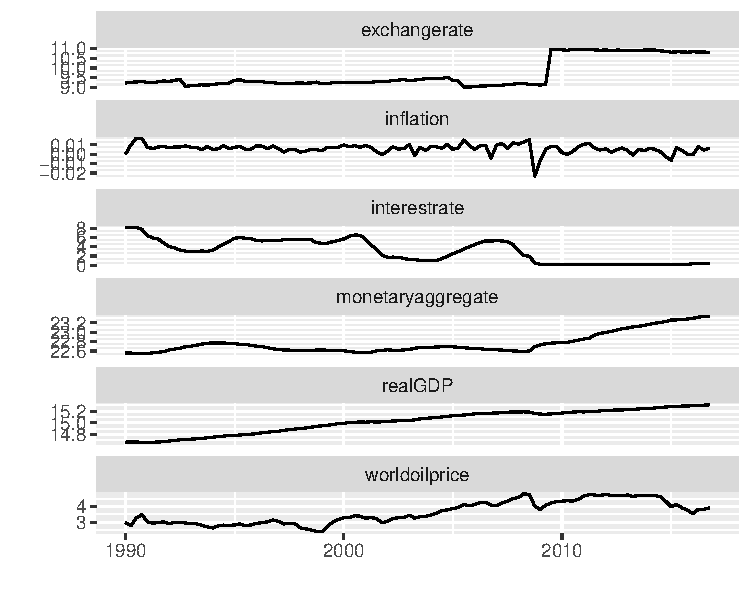
\includegraphics{README_files/figure-latex/unnamed-chunk-1-1} \end{center}

\begin{verbatim}
## AIC(n)  HQ(n)  SC(n) FPE(n) 
##      9      3      1      4
\end{verbatim}

\begin{verbatim}
## AIC(n)  HQ(n)  SC(n) FPE(n) 
##      9      3      1      4
\end{verbatim}

Use AIC and find that lag should be 2 according to the paper, but we
find AIC suggests 9 so we use 8\ldots overparameterised\ldots{}

\hypertarget{step-4-johansen-test-in-the-long-run-approach}{%
\section{Step 4: Johansen Test in the Long-Run
Approach}\label{step-4-johansen-test-in-the-long-run-approach}}

\begin{verbatim}
## 
## ###################### 
## # Johansen-Procedure # 
## ###################### 
## 
## Test type: maximal eigenvalue statistic (lambda max) , with linear trend in cointegration 
## 
## Eigenvalues (lambda):
## [1]  3.979695e-01  3.042675e-01  2.153416e-01  9.738484e-02  3.505572e-02
## [6] -1.178400e-16
## 
## Values of teststatistic and critical values of test:
## 
##           test 10pct  5pct  1pct
## r <= 4 |  3.78 10.49 12.25 16.26
## r <= 3 | 10.86 16.85 18.96 23.65
## r <= 2 | 25.71 23.11 25.54 30.34
## r <= 1 | 38.46 29.12 31.46 36.65
## r = 0  | 53.79 34.75 37.52 42.36
## 
## Eigenvectors, normalised to first column:
## (These are the cointegration relations)
## 
##                      InterestRate.l2 Inflation.l2  RealGDP.l2
## InterestRate.l2            1.0000000   1.00000000   1.0000000
## Inflation.l2           -2031.1972531  60.14611922  83.9230204
## RealGDP.l2                44.3664771  91.40333932 -61.2150997
## MonetaryAggregate.l2      -2.1675253  13.84339202  -9.0304301
## ExchangeRate.l2            3.9947077   4.12487201  -4.1440037
## trend.l2                  -0.1098671  -0.04984123   0.1212989
##                      MonetaryAggregate.l2 ExchangeRate.l2    trend.l2
## InterestRate.l2                1.00000000        1.000000   1.0000000
## Inflation.l2                -104.04152982     -186.801057  67.9822906
## RealGDP.l2                   -63.95611350     1116.457893 -51.9615009
## MonetaryAggregate.l2         -22.52197056      133.718072  23.3950513
## ExchangeRate.l2                4.11789111        5.345720  -4.5260646
## trend.l2                       0.01077267        1.113211   0.1991169
## 
## Weights W:
## (This is the loading matrix)
## 
##                     InterestRate.l2  Inflation.l2    RealGDP.l2
## InterestRate.d         0.0078295417 -2.829900e-02 -3.016202e-02
## Inflation.d            0.0005179529  3.106081e-05  4.416704e-05
## RealGDP.d              0.0001337988  1.001147e-04 -6.358223e-04
## MonetaryAggregate.d   -0.0007028248 -1.739070e-03 -1.169081e-03
## ExchangeRate.d         0.0022638988 -3.169329e-02  3.217220e-02
##                     MonetaryAggregate.l2 ExchangeRate.l2      trend.l2
## InterestRate.d             -2.801371e-02    3.369312e-04  3.753628e-17
## Inflation.d                -1.714724e-05    2.817733e-06 -1.609146e-18
## RealGDP.d                  -2.760986e-04   -1.743527e-05 -3.191874e-18
## MonetaryAggregate.d         9.917425e-04    2.214224e-06  3.888824e-20
## ExchangeRate.d             -2.983729e-03   -2.378842e-04  2.750099e-16
\end{verbatim}

\begin{verbatim}
## 
## ###################### 
## # Johansen-Procedure # 
## ###################### 
## 
## Test type: trace statistic , with linear trend in cointegration 
## 
## Eigenvalues (lambda):
## [1]  3.979695e-01  3.042675e-01  2.153416e-01  9.738484e-02  3.505572e-02
## [6] -1.178400e-16
## 
## Values of teststatistic and critical values of test:
## 
##            test 10pct  5pct  1pct
## r <= 4 |   3.78 10.49 12.25 16.26
## r <= 3 |  14.64 22.76 25.32 30.45
## r <= 2 |  40.35 39.06 42.44 48.45
## r <= 1 |  78.80 59.14 62.99 70.05
## r = 0  | 132.59 83.20 87.31 96.58
## 
## Eigenvectors, normalised to first column:
## (These are the cointegration relations)
## 
##                      InterestRate.l2 Inflation.l2  RealGDP.l2
## InterestRate.l2            1.0000000   1.00000000   1.0000000
## Inflation.l2           -2031.1972531  60.14611922  83.9230204
## RealGDP.l2                44.3664771  91.40333932 -61.2150997
## MonetaryAggregate.l2      -2.1675253  13.84339202  -9.0304301
## ExchangeRate.l2            3.9947077   4.12487201  -4.1440037
## trend.l2                  -0.1098671  -0.04984123   0.1212989
##                      MonetaryAggregate.l2 ExchangeRate.l2    trend.l2
## InterestRate.l2                1.00000000        1.000000   1.0000000
## Inflation.l2                -104.04152982     -186.801057  67.9822906
## RealGDP.l2                   -63.95611350     1116.457893 -51.9615009
## MonetaryAggregate.l2         -22.52197056      133.718072  23.3950513
## ExchangeRate.l2                4.11789111        5.345720  -4.5260646
## trend.l2                       0.01077267        1.113211   0.1991169
## 
## Weights W:
## (This is the loading matrix)
## 
##                     InterestRate.l2  Inflation.l2    RealGDP.l2
## InterestRate.d         0.0078295417 -2.829900e-02 -3.016202e-02
## Inflation.d            0.0005179529  3.106081e-05  4.416704e-05
## RealGDP.d              0.0001337988  1.001147e-04 -6.358223e-04
## MonetaryAggregate.d   -0.0007028248 -1.739070e-03 -1.169081e-03
## ExchangeRate.d         0.0022638988 -3.169329e-02  3.217220e-02
##                     MonetaryAggregate.l2 ExchangeRate.l2      trend.l2
## InterestRate.d             -2.801371e-02    3.369312e-04  3.753628e-17
## Inflation.d                -1.714724e-05    2.817733e-06 -1.609146e-18
## RealGDP.d                  -2.760986e-04   -1.743527e-05 -3.191874e-18
## MonetaryAggregate.d         9.917425e-04    2.214224e-06  3.888824e-20
## ExchangeRate.d             -2.983729e-03   -2.378842e-04  2.750099e-16
\end{verbatim}

Intially found that matrix was computationally singular, therefore,
needed to change matrix so it could be invertible.

Let us check for multicollinearity

\begin{verbatim}
##                   InterestRate Inflation RealGDP MonetaryAggregate ExchangeRate
## InterestRate              1.00      0.33    0.26             -0.16        -0.74
## Inflation                 0.33      1.00    0.14             -0.14        -0.20
## RealGDP                   0.26      0.14    1.00             -0.81        -0.51
## MonetaryAggregate        -0.16     -0.14   -0.81              1.00         0.42
## ExchangeRate             -0.74     -0.20   -0.51              0.42         1.00
## 
## n= 108 
## 
## 
## P
##                   InterestRate Inflation RealGDP MonetaryAggregate ExchangeRate
## InterestRate                   0.0005    0.0061  0.0882            0.0000      
## Inflation         0.0005                 0.1358  0.1606            0.0394      
## RealGDP           0.0061       0.1358            0.0000            0.0000      
## MonetaryAggregate 0.0882       0.1606    0.0000                    0.0000      
## ExchangeRate      0.0000       0.0394    0.0000  0.0000
\end{verbatim}

ALL STATISTICALLY SIGNIFICANTLY CORRELATED

Tried to test correlation if did not transform monetary aggregate and
inflation as paper did, but still highly correlated.

For the eigenvalue test, we find that we can reject the null hypothesis
of the number of cointegrating relationships equalling 2 or exceeding
it, therefore, we conclude from our estimates that there is one
cointegrating relationship.

We obtain the cointegrating vectors from the Johansen test using: You
can extract the cointegrating vectors by addressing the slot V by
(\textbf{V?}) like \href{mailto:sjd.vecm@V}{\nolinkurl{sjd.vecm@V}}.
This will be a matrix where each column is a cointegrating vector. You
can multiply the original multivariate series (like sjd) to the V matrix
to get the error correction terms.

Check if the cointegrating relationships are trending and not random
walks, show graphically the cointegrating vectors

\begin{center}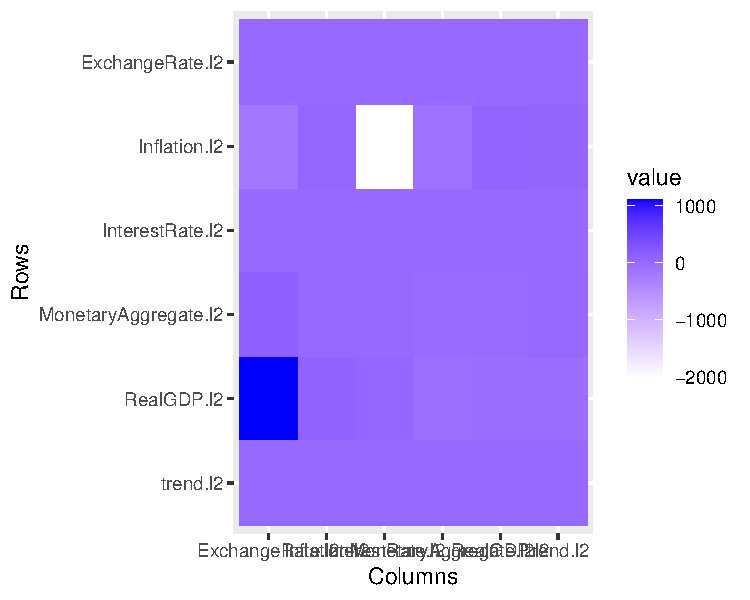
\includegraphics{README_files/figure-latex/unnamed-chunk-10-1} \end{center}

\hypertarget{step-3-augemented-dickey-fuller-tests}{%
\section{Step 3: Augemented Dickey-Fuller
tests}\label{step-3-augemented-dickey-fuller-tests}}

The null-hypothesis of an Augmented Dickey-Fuller test is that the
series has a unit-root. We ask, is the estimated critical value small
enough to reject the null-hypothesis? If yes, we cannot reject the null
hypothesis, therefore, the series may be non-stationary.

In this section, we find that the interest rate is stationary, change in
inflation is stationary, detrended real GDP is still not stationary,
detrended monetary aggregate is still non-stationary and world oil price
is non stationary.

Interest Rate

\begin{center}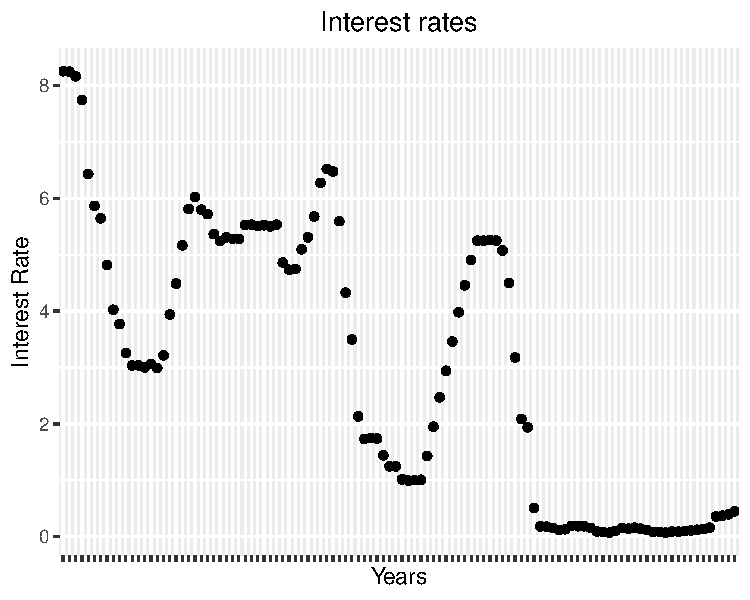
\includegraphics{README_files/figure-latex/unnamed-chunk-12-1} \end{center}

The estimated critical value for the Augmented Dickey Fuller test for
the interest rate is small enough to reject the null hypothesis at 5\%
confidence interval = -2.2403\textless-1.95, therefore, may be a
stationary series.

\begin{center}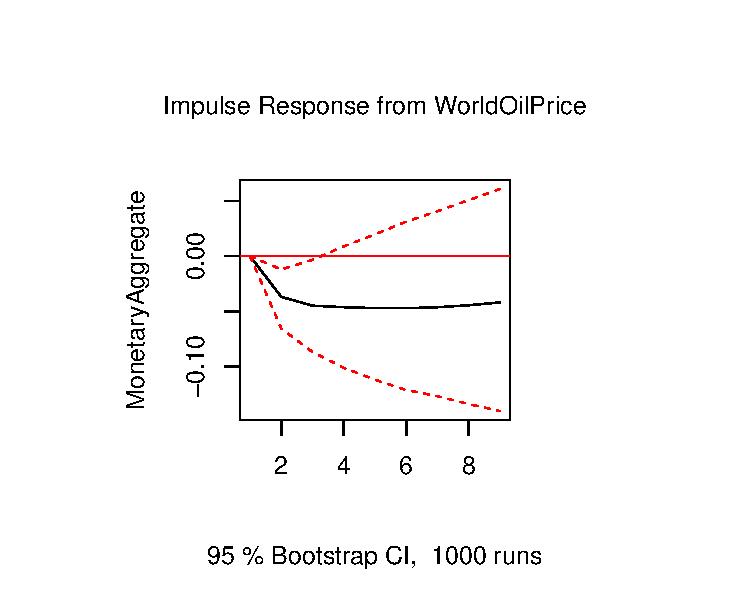
\includegraphics{README_files/figure-latex/unnamed-chunk-13-1} \end{center}

The estimated critical value of -3.4624 for inflation is small enough to
reject the null hypothesis at 1\% confidence interval,
-3.4624\textless-2.58. Therefore can reject the null hypothesis that
there is a unit root and series may be stationary.

\begin{center}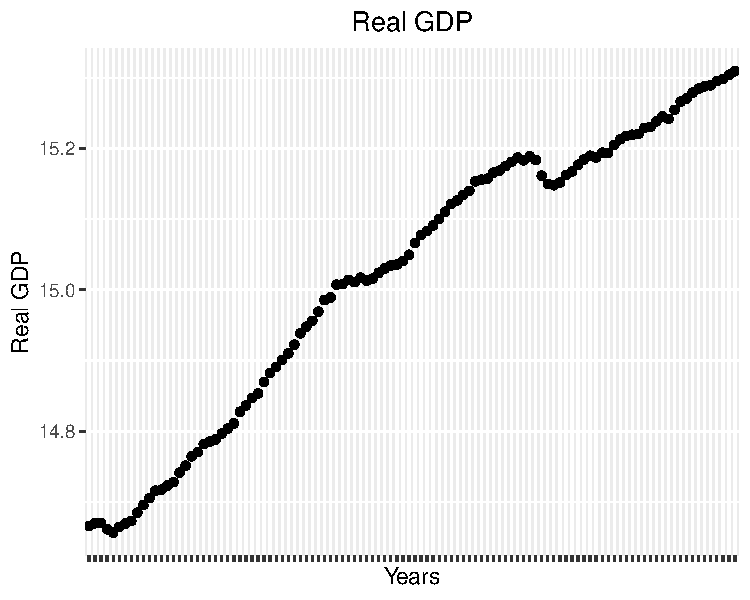
\includegraphics{README_files/figure-latex/unnamed-chunk-14-1} \end{center}

Think we should detrend, because seems to be a clear upward linear trend

\begin{center}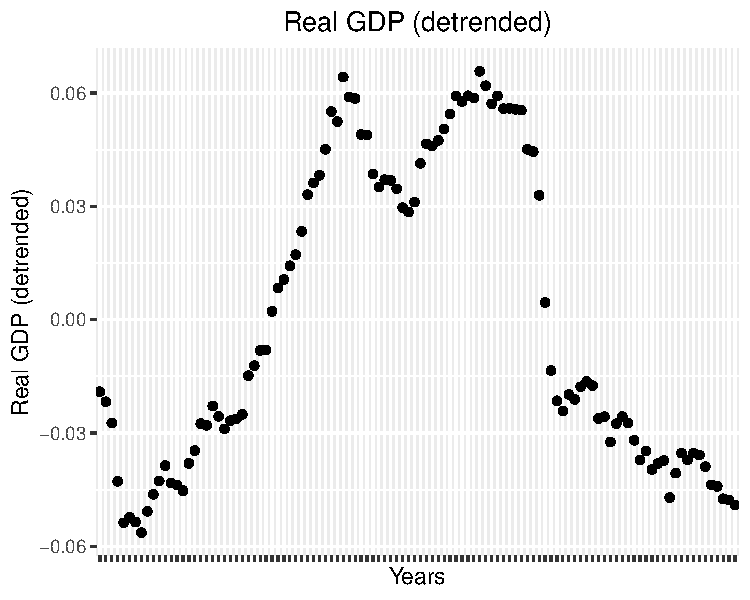
\includegraphics{README_files/figure-latex/unnamed-chunk-15-1} \end{center}

Detrended Real GDP series is still non-stationary. But cannot first
difference it in case remove important information.

\begin{center}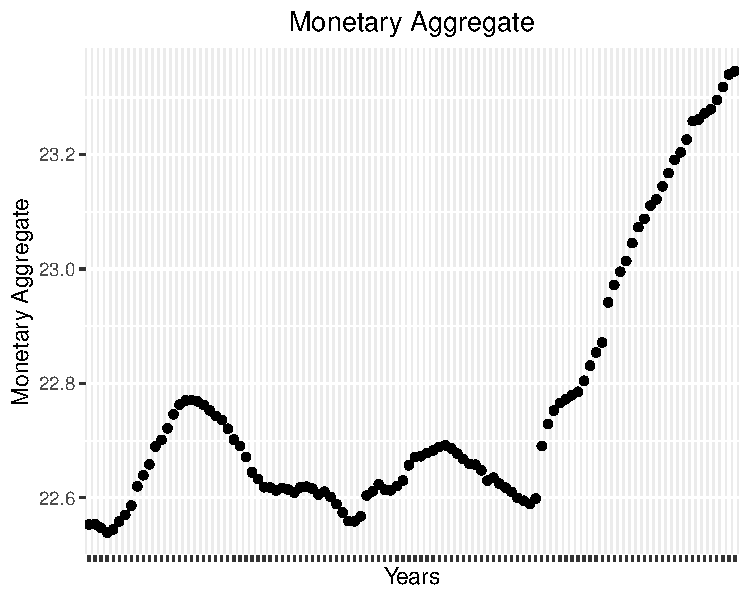
\includegraphics{README_files/figure-latex/unnamed-chunk-18-1} \end{center}

No clear trend for the Transformed Monetary Aggregate\ldots try
difference? cannot because then all values go to zero

Think we should detrend, because seems to be a clear upward linear trend

\begin{center}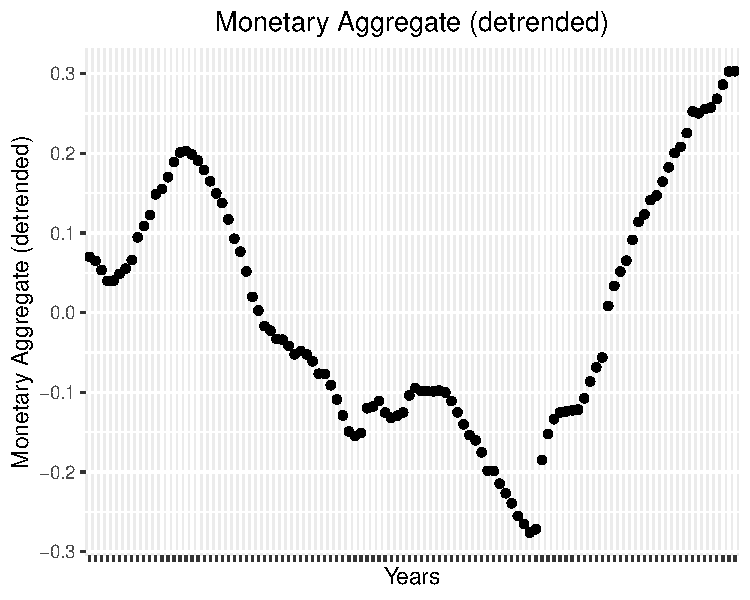
\includegraphics{README_files/figure-latex/unnamed-chunk-19-1} \end{center}

Detrended Monetary Aggregate is still non-stationary because cannot
reject null hypothesis.

\begin{center}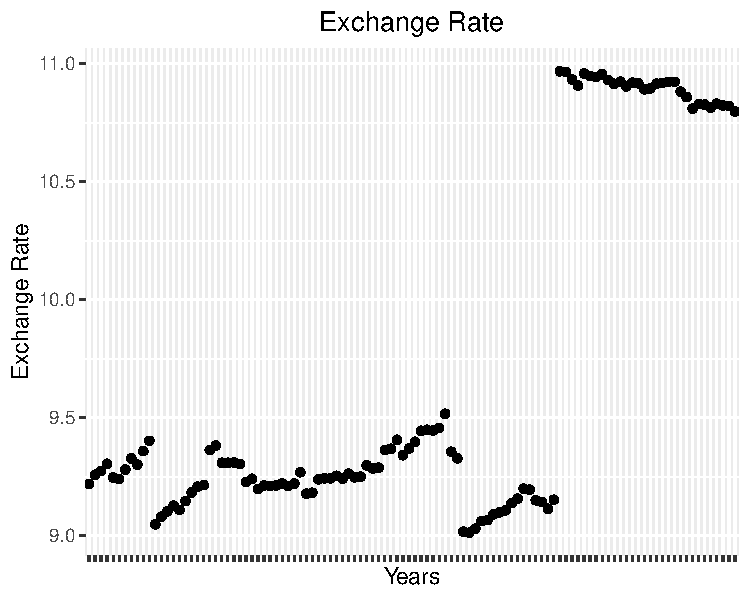
\includegraphics{README_files/figure-latex/unnamed-chunk-20-1} \end{center}

Let us try first difference the exchange rate.

This does not work because it makes the series have no variation,
removes too much information.

\begin{center}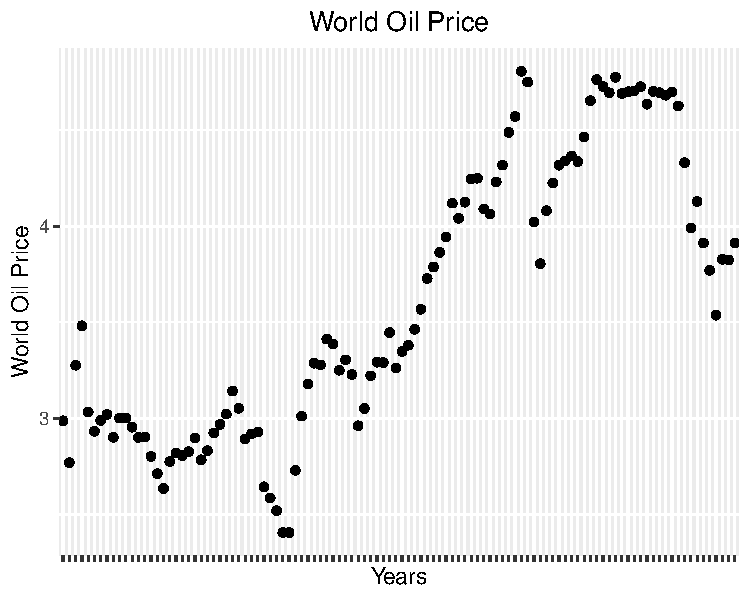
\includegraphics{README_files/figure-latex/unnamed-chunk-22-1} \end{center}

\begin{verbatim}
## 
## ############################################### 
## # Augmented Dickey-Fuller Test Unit Root Test # 
## ############################################### 
## 
## Test regression none 
## 
## 
## Call:
## lm(formula = z.diff ~ z.lag.1 - 1 + z.diff.lag)
## 
## Residuals:
##      Min       1Q   Median       3Q      Max 
## -1.30124 -0.04024  0.03284  0.19765  0.64002 
## 
## Coefficients:
##             Estimate Std. Error t value Pr(>|t|)    
## z.lag.1    -0.017754   0.007925  -2.240   0.0272 *  
## z.diff.lag  0.665828   0.070243   9.479 9.82e-16 ***
## ---
## Signif. codes:  0 '***' 0.001 '**' 0.01 '*' 0.05 '.' 0.1 ' ' 1
## 
## Residual standard error: 0.3117 on 104 degrees of freedom
## Multiple R-squared:  0.4962, Adjusted R-squared:  0.4865 
## F-statistic: 51.22 on 2 and 104 DF,  p-value: 3.283e-16
## 
## 
## Value of test-statistic is: -2.2403 
## 
## Critical values for test statistics: 
##       1pct  5pct 10pct
## tau1 -2.58 -1.95 -1.62
\end{verbatim}

\begin{verbatim}
## 
## ############################################### 
## # Augmented Dickey-Fuller Test Unit Root Test # 
## ############################################### 
## 
## Test regression none 
## 
## 
## Call:
## lm(formula = z.diff ~ z.lag.1 - 1 + z.diff.lag)
## 
## Residuals:
##       Min        1Q    Median        3Q       Max 
## -0.034171 -0.000633  0.002036  0.004299  0.012676 
## 
## Coefficients:
##            Estimate Std. Error t value Pr(>|t|)    
## z.lag.1    -0.25933    0.07490  -3.462 0.000778 ***
## z.diff.lag -0.13897    0.09595  -1.448 0.150533    
## ---
## Signif. codes:  0 '***' 0.001 '**' 0.01 '*' 0.05 '.' 0.1 ' ' 1
## 
## Residual standard error: 0.005504 on 104 degrees of freedom
## Multiple R-squared:  0.1699, Adjusted R-squared:  0.154 
## F-statistic: 10.65 on 2 and 104 DF,  p-value: 6.221e-05
## 
## 
## Value of test-statistic is: -3.4624 
## 
## Critical values for test statistics: 
##       1pct  5pct 10pct
## tau1 -2.58 -1.95 -1.62
\end{verbatim}

Real GDP

\begin{verbatim}
## 
## ############################################### 
## # Augmented Dickey-Fuller Test Unit Root Test # 
## ############################################### 
## 
## Test regression none 
## 
## 
## Call:
## lm(formula = z.diff ~ z.lag.1 - 1 + z.diff.lag)
## 
## Residuals:
##        Min         1Q     Median         3Q        Max 
## -0.0231012 -0.0033550  0.0003949  0.0032334  0.0135407 
## 
## Coefficients:
##            Estimate Std. Error t value Pr(>|t|)    
## z.lag.1    -0.01298    0.01361  -0.954    0.342    
## z.diff.lag  0.41772    0.08963   4.660 9.39e-06 ***
## ---
## Signif. codes:  0 '***' 0.001 '**' 0.01 '*' 0.05 '.' 0.1 ' ' 1
## 
## Residual standard error: 0.005569 on 104 degrees of freedom
## Multiple R-squared:  0.174,  Adjusted R-squared:  0.1581 
## F-statistic: 10.95 on 2 and 104 DF,  p-value: 4.829e-05
## 
## 
## Value of test-statistic is: -0.9539 
## 
## Critical values for test statistics: 
##       1pct  5pct 10pct
## tau1 -2.58 -1.95 -1.62
\end{verbatim}

Monetary Aggregates

\begin{verbatim}
## 
## ############################################### 
## # Augmented Dickey-Fuller Test Unit Root Test # 
## ############################################### 
## 
## Test regression none 
## 
## 
## Call:
## lm(formula = z.diff ~ z.lag.1 - 1 + z.diff.lag)
## 
## Residuals:
##       Min        1Q    Median        3Q       Max 
## -0.023625 -0.006963 -0.001197  0.006941  0.082536 
## 
## Coefficients:
##             Estimate Std. Error t value Pr(>|t|)    
## z.lag.1    -0.005069   0.009301  -0.545    0.587    
## z.diff.lag  0.642516   0.077496   8.291 4.24e-13 ***
## ---
## Signif. codes:  0 '***' 0.001 '**' 0.01 '*' 0.05 '.' 0.1 ' ' 1
## 
## Residual standard error: 0.01395 on 104 degrees of freedom
## Multiple R-squared:  0.4033, Adjusted R-squared:  0.3919 
## F-statistic: 35.15 on 2 and 104 DF,  p-value: 2.177e-12
## 
## 
## Value of test-statistic is: -0.545 
## 
## Critical values for test statistics: 
##       1pct  5pct 10pct
## tau1 -2.58 -1.95 -1.62
\end{verbatim}

Exchange Rate

\begin{verbatim}
## 
## ############################################### 
## # Augmented Dickey-Fuller Test Unit Root Test # 
## ############################################### 
## 
## Test regression none 
## 
## 
## Call:
## lm(formula = z.diff ~ z.lag.1 - 1 + z.diff.lag)
## 
## Residuals:
##      Min       1Q   Median       3Q      Max 
## -0.36660 -0.02652 -0.00900  0.01104  1.80232 
## 
## Coefficients:
##            Estimate Std. Error t value Pr(>|t|)
## z.lag.1    0.001348   0.001877   0.718    0.474
## z.diff.lag 0.005283   0.098225   0.054    0.957
## 
## Residual standard error: 0.187 on 104 degrees of freedom
## Multiple R-squared:  0.005078,   Adjusted R-squared:  -0.01406 
## F-statistic: 0.2654 on 2 and 104 DF,  p-value: 0.7674
## 
## 
## Value of test-statistic is: 0.7184 
## 
## Critical values for test statistics: 
##       1pct  5pct 10pct
## tau1 -2.58 -1.95 -1.62
\end{verbatim}

0.0214 \textgreater-2.6 therefore cannot reject the unit root

World Oil Price

\begin{verbatim}
## 
## ############################################### 
## # Augmented Dickey-Fuller Test Unit Root Test # 
## ############################################### 
## 
## Test regression none 
## 
## 
## Call:
## lm(formula = z.diff ~ z.lag.1 - 1 + z.diff.lag)
## 
## Residuals:
##      Min       1Q   Median       3Q      Max 
## -0.72572 -0.06453  0.01614  0.08600  0.53844 
## 
## Coefficients:
##            Estimate Std. Error t value Pr(>|t|)  
## z.lag.1    0.001240   0.004215   0.294    0.769  
## z.diff.lag 0.160192   0.096223   1.665    0.099 .
## ---
## Signif. codes:  0 '***' 0.001 '**' 0.01 '*' 0.05 '.' 0.1 ' ' 1
## 
## Residual standard error: 0.1595 on 104 degrees of freedom
## Multiple R-squared:  0.02747,    Adjusted R-squared:  0.008763 
## F-statistic: 1.469 on 2 and 104 DF,  p-value: 0.235
## 
## 
## Value of test-statistic is: 0.2942 
## 
## Critical values for test statistics: 
##       1pct  5pct 10pct
## tau1 -2.58 -1.95 -1.62
\end{verbatim}

\hypertarget{set-up-the-var-model}{%
\section{Set up the VAR model}\label{set-up-the-var-model}}

\hypertarget{acf-pacf}{%
\subsection{ACF \& PACF}\label{acf-pacf}}

\begin{center}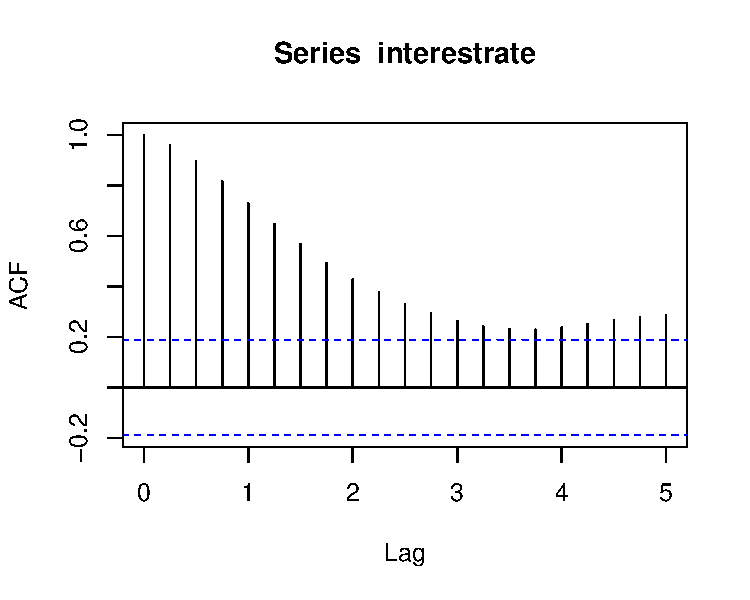
\includegraphics{README_files/figure-latex/unnamed-chunk-29-1} \end{center}

\begin{center}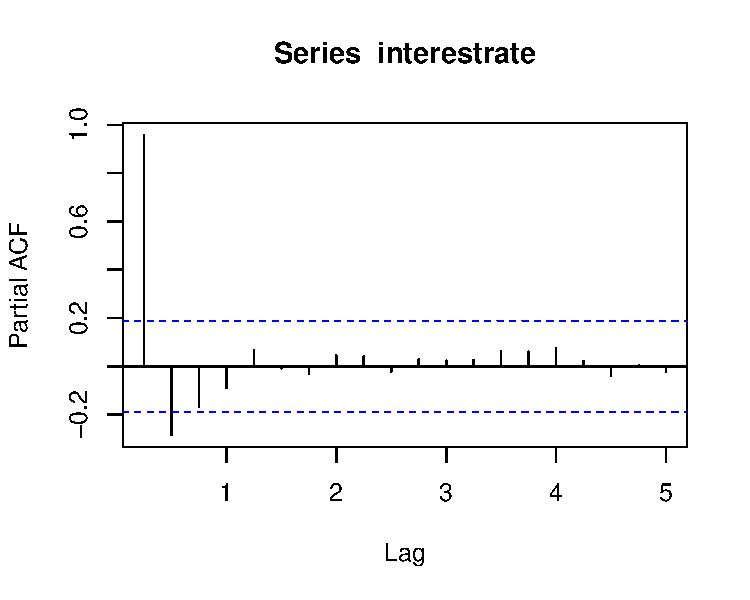
\includegraphics{README_files/figure-latex/unnamed-chunk-29-2} \end{center}

Interest rate autocorrelation function shows that 5 lags are
significant. Partial autocorrelation function shows less than one lag is
significant.

\begin{center}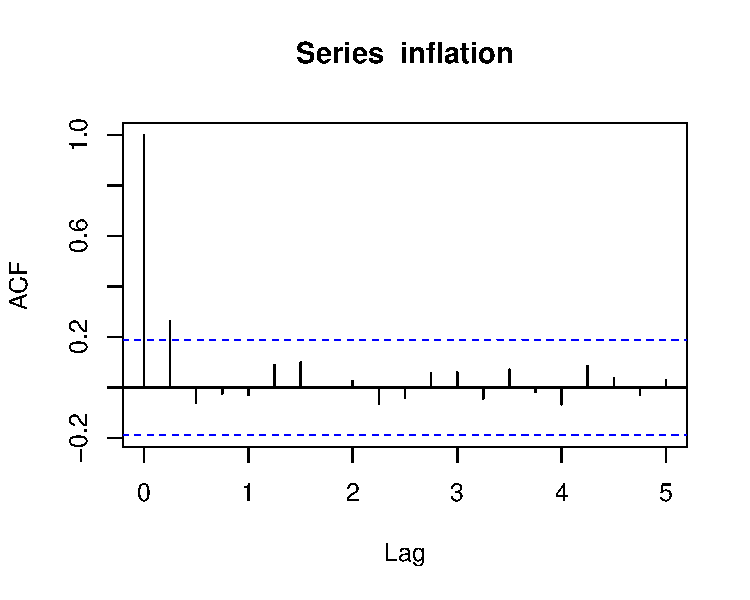
\includegraphics{README_files/figure-latex/unnamed-chunk-30-1} \end{center}

\begin{center}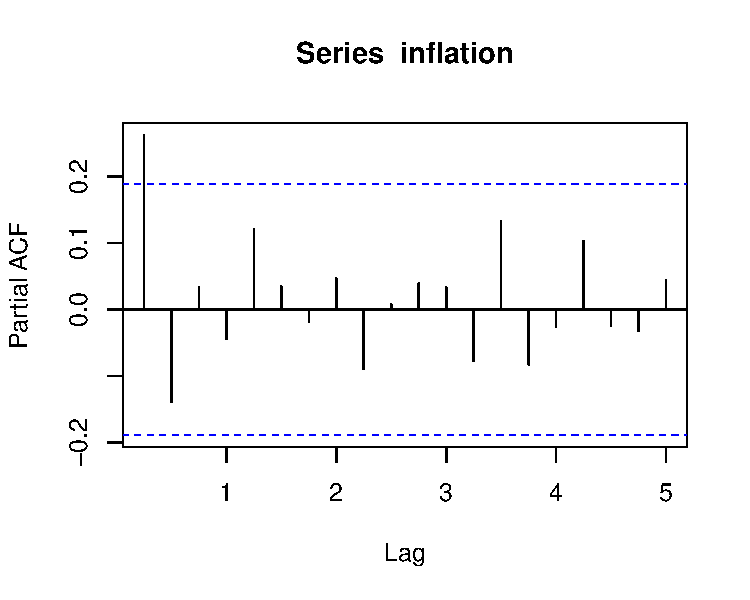
\includegraphics{README_files/figure-latex/unnamed-chunk-30-2} \end{center}

Cannot find significant lags for inflation for autocorrelation function
or partial autocorrelation function.

\begin{center}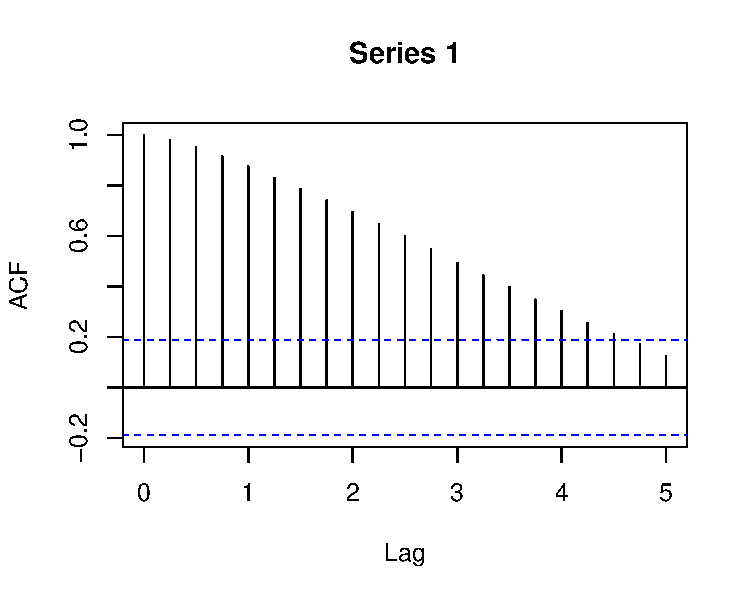
\includegraphics{README_files/figure-latex/unnamed-chunk-31-1} \end{center}

\begin{center}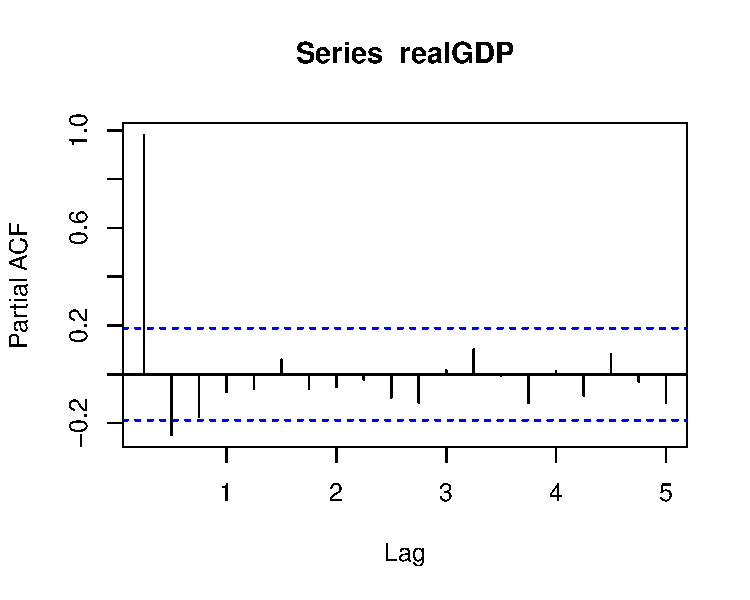
\includegraphics{README_files/figure-latex/unnamed-chunk-31-2} \end{center}

Real GDP is significant up to 5 lags showing lots of persistence and
partial autocorrelation function shows significance for less than one
lag, at one quarter only.

\begin{center}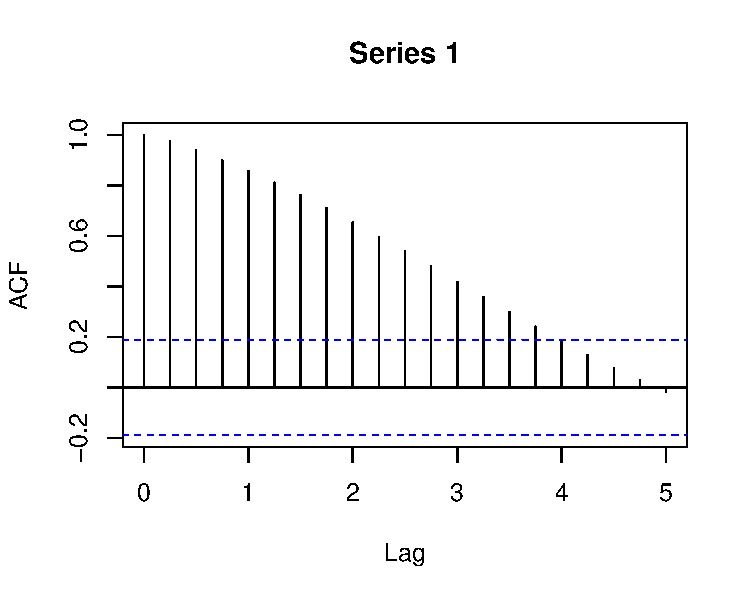
\includegraphics{README_files/figure-latex/unnamed-chunk-32-1} \end{center}

\begin{center}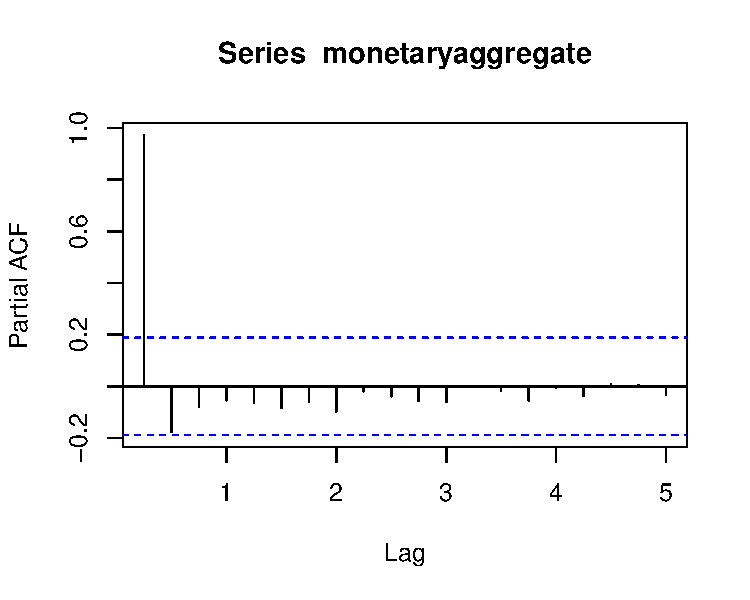
\includegraphics{README_files/figure-latex/unnamed-chunk-32-2} \end{center}

Monetary aggregate's autocorrelation function indicates that lags up to
5 are significant and partial autocorrelation function shows only first
quarter significant.

\begin{center}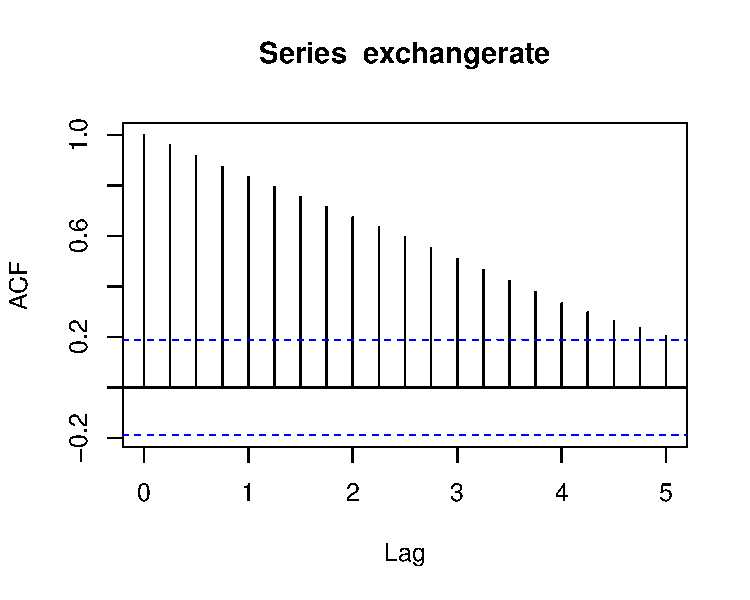
\includegraphics{README_files/figure-latex/unnamed-chunk-33-1} \end{center}

\begin{center}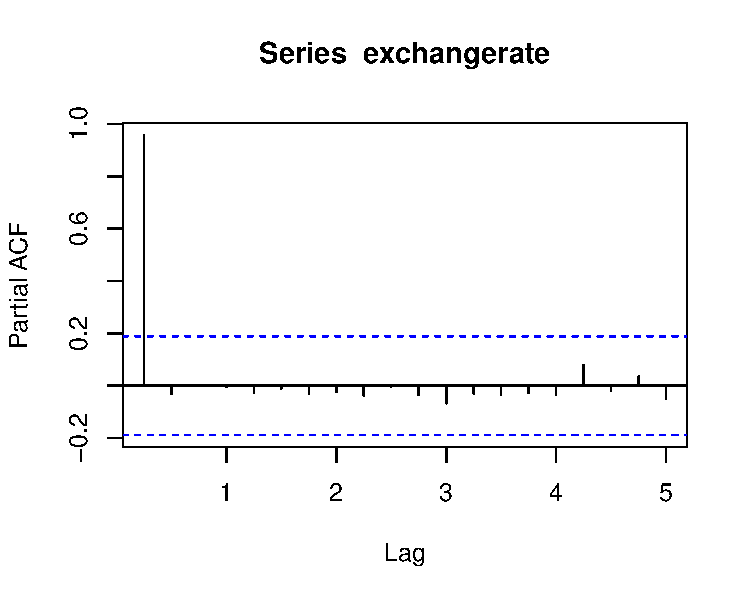
\includegraphics{README_files/figure-latex/unnamed-chunk-33-2} \end{center}

Autocorrelation function for exchange rate indicates significance up to
lag 4 and partial autocorrelation shows only first quarter significant.

\begin{center}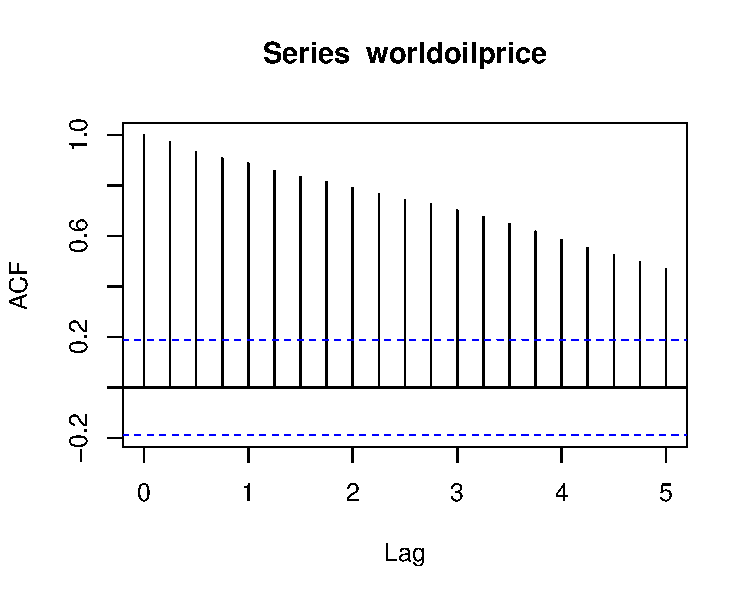
\includegraphics{README_files/figure-latex/unnamed-chunk-34-1} \end{center}

\begin{center}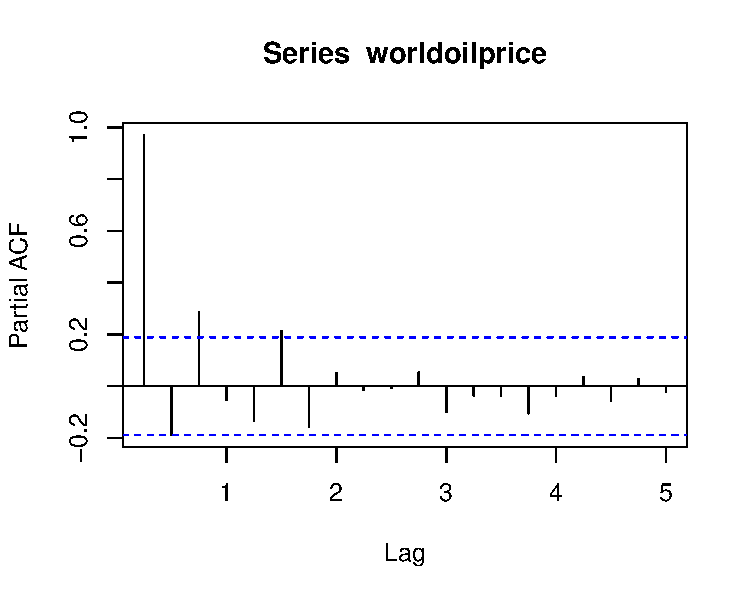
\includegraphics{README_files/figure-latex/unnamed-chunk-34-2} \end{center}

\hypertarget{build-model}{%
\subsection{Build model}\label{build-model}}

\begin{verbatim}
## 
## VAR Estimation Results:
## ========================= 
## Endogenous variables: InterestRate, Inflation, RealGDP, MonetaryAggregate, ExchangeRate 
## Deterministic variables: trend 
## Sample size: 105 
## Log Likelihood: 1248.331 
## Roots of the characteristic polynomial:
## 1.012 0.9708 0.8984 0.8984 0.8336 0.663 0.663 0.6347 0.6347 0.5873 0.5873 0.4406 0.262 0.262 0.004563
## Call:
## VAR(y = groupedVARendog, p = 3, type = "trend", exogen = NULL)
## 
## 
## Estimation results for equation InterestRate: 
## ============================================= 
## InterestRate = InterestRate.l1 + Inflation.l1 + RealGDP.l1 + MonetaryAggregate.l1 + ExchangeRate.l1 + InterestRate.l2 + Inflation.l2 + RealGDP.l2 + MonetaryAggregate.l2 + ExchangeRate.l2 + InterestRate.l3 + Inflation.l3 + RealGDP.l3 + MonetaryAggregate.l3 + ExchangeRate.l3 + trend 
## 
##                        Estimate Std. Error t value Pr(>|t|)    
## InterestRate.l1        1.423110   0.111934  12.714  < 2e-16 ***
## Inflation.l1         -15.817420   7.568504  -2.090  0.03948 *  
## RealGDP.l1            14.308641   5.753821   2.487  0.01475 *  
## MonetaryAggregate.l1  -0.809772   3.071928  -0.264  0.79269    
## ExchangeRate.l1       -0.020080   0.163901  -0.123  0.90277    
## InterestRate.l2       -0.304428   0.189497  -1.607  0.11171    
## Inflation.l2          -3.117641   8.058570  -0.387  0.69977    
## RealGDP.l2           -20.584455   9.028203  -2.280  0.02500 *  
## MonetaryAggregate.l2   2.163174   5.012847   0.432  0.66713    
## ExchangeRate.l2        0.055810   0.220709   0.253  0.80095    
## InterestRate.l3       -0.207443   0.104840  -1.979  0.05095 .  
## Inflation.l3           1.668348   6.583085   0.253  0.80052    
## RealGDP.l3            10.003101   6.052027   1.653  0.10188    
## MonetaryAggregate.l3  -0.759100   3.000095  -0.253  0.80083    
## ExchangeRate.l3        0.039071   0.161173   0.242  0.80902    
## trend                 -0.006744   0.002212  -3.049  0.00303 ** 
## ---
## Signif. codes:  0 '***' 0.001 '**' 0.01 '*' 0.05 '.' 0.1 ' ' 1
## 
## 
## Residual standard error: 0.2876 on 89 degrees of freedom
## Multiple R-Squared: 0.9949,  Adjusted R-squared: 0.994 
## F-statistic:  1083 on 16 and 89 DF,  p-value: < 2.2e-16 
## 
## 
## Estimation results for equation Inflation: 
## ========================================== 
## Inflation = InterestRate.l1 + Inflation.l1 + RealGDP.l1 + MonetaryAggregate.l1 + ExchangeRate.l1 + InterestRate.l2 + Inflation.l2 + RealGDP.l2 + MonetaryAggregate.l2 + ExchangeRate.l2 + InterestRate.l3 + Inflation.l3 + RealGDP.l3 + MonetaryAggregate.l3 + ExchangeRate.l3 + trend 
## 
##                        Estimate Std. Error t value Pr(>|t|)  
## InterestRate.l1      -1.653e-03  1.804e-03  -0.916   0.3621  
## Inflation.l1          2.008e-01  1.220e-01   1.646   0.1034  
## RealGDP.l1            1.474e-01  9.275e-02   1.589   0.1155  
## MonetaryAggregate.l1 -6.013e-03  4.952e-02  -0.121   0.9036  
## ExchangeRate.l1       1.651e-03  2.642e-03   0.625   0.5335  
## InterestRate.l2       5.364e-03  3.055e-03   1.756   0.0825 .
## Inflation.l2         -1.977e-01  1.299e-01  -1.522   0.1316  
## RealGDP.l2           -2.199e-01  1.455e-01  -1.511   0.1344  
## MonetaryAggregate.l2  3.405e-02  8.081e-02   0.421   0.6745  
## ExchangeRate.l2      -3.688e-03  3.558e-03  -1.037   0.3027  
## InterestRate.l3      -3.435e-03  1.690e-03  -2.033   0.0451 *
## Inflation.l3         -3.753e-02  1.061e-01  -0.354   0.7245  
## RealGDP.l3            8.373e-02  9.756e-02   0.858   0.3931  
## MonetaryAggregate.l3 -3.182e-02  4.836e-02  -0.658   0.5123  
## ExchangeRate.l3       2.854e-03  2.598e-03   1.098   0.2750  
## trend                -4.709e-05  3.566e-05  -1.321   0.1900  
## ---
## Signif. codes:  0 '***' 0.001 '**' 0.01 '*' 0.05 '.' 0.1 ' ' 1
## 
## 
## Residual standard error: 0.004637 on 89 degrees of freedom
## Multiple R-Squared: 0.6827,  Adjusted R-squared: 0.6256 
## F-statistic: 11.97 on 16 and 89 DF,  p-value: 6.085e-16 
## 
## 
## Estimation results for equation RealGDP: 
## ======================================== 
## RealGDP = InterestRate.l1 + Inflation.l1 + RealGDP.l1 + MonetaryAggregate.l1 + ExchangeRate.l1 + InterestRate.l2 + Inflation.l2 + RealGDP.l2 + MonetaryAggregate.l2 + ExchangeRate.l2 + InterestRate.l3 + Inflation.l3 + RealGDP.l3 + MonetaryAggregate.l3 + ExchangeRate.l3 + trend 
## 
##                        Estimate Std. Error t value Pr(>|t|)    
## InterestRate.l1      -2.789e-03  2.118e-03  -1.317   0.1912    
## Inflation.l1         -1.748e-01  1.432e-01  -1.221   0.2255    
## RealGDP.l1            1.270e+00  1.089e-01  11.667   <2e-16 ***
## MonetaryAggregate.l1 -5.572e-02  5.812e-02  -0.959   0.3402    
## ExchangeRate.l1       4.232e-03  3.101e-03   1.365   0.1757    
## InterestRate.l2       5.900e-03  3.585e-03   1.646   0.1034    
## Inflation.l2         -1.381e-01  1.525e-01  -0.906   0.3675    
## RealGDP.l2           -8.884e-02  1.708e-01  -0.520   0.6043    
## MonetaryAggregate.l2  1.028e-01  9.483e-02   1.084   0.2811    
## ExchangeRate.l2      -5.183e-03  4.175e-03  -1.241   0.2178    
## InterestRate.l3      -3.710e-03  1.983e-03  -1.870   0.0647 .  
## Inflation.l3         -3.322e-02  1.245e-01  -0.267   0.7903    
## RealGDP.l3           -1.665e-01  1.145e-01  -1.454   0.1494    
## MonetaryAggregate.l3 -4.413e-02  5.676e-02  -0.778   0.4389    
## ExchangeRate.l3       1.902e-03  3.049e-03   0.624   0.5343    
## trend                -9.561e-05  4.185e-05  -2.285   0.0247 *  
## ---
## Signif. codes:  0 '***' 0.001 '**' 0.01 '*' 0.05 '.' 0.1 ' ' 1
## 
## 
## Residual standard error: 0.005442 on 89 degrees of freedom
## Multiple R-Squared: 0.9846,  Adjusted R-squared: 0.9818 
## F-statistic: 355.1 on 16 and 89 DF,  p-value: < 2.2e-16 
## 
## 
## Estimation results for equation MonetaryAggregate: 
## ================================================== 
## MonetaryAggregate = InterestRate.l1 + Inflation.l1 + RealGDP.l1 + MonetaryAggregate.l1 + ExchangeRate.l1 + InterestRate.l2 + Inflation.l2 + RealGDP.l2 + MonetaryAggregate.l2 + ExchangeRate.l2 + InterestRate.l3 + Inflation.l3 + RealGDP.l3 + MonetaryAggregate.l3 + ExchangeRate.l3 + trend 
## 
##                        Estimate Std. Error t value Pr(>|t|)    
## InterestRate.l1      -3.702e-03  4.783e-03  -0.774   0.4410    
## Inflation.l1          7.937e-01  3.234e-01   2.454   0.0161 *  
## RealGDP.l1           -2.688e-01  2.459e-01  -1.093   0.2771    
## MonetaryAggregate.l1  1.307e+00  1.313e-01   9.956 3.94e-16 ***
## ExchangeRate.l1      -7.662e-03  7.003e-03  -1.094   0.2769    
## InterestRate.l2      -3.578e-03  8.097e-03  -0.442   0.6596    
## Inflation.l2          4.394e-01  3.443e-01   1.276   0.2053    
## RealGDP.l2           -3.323e-02  3.858e-01  -0.086   0.9315    
## MonetaryAggregate.l2 -3.311e-01  2.142e-01  -1.546   0.1257    
## ExchangeRate.l2      -2.519e-03  9.431e-03  -0.267   0.7900    
## InterestRate.l3       4.590e-03  4.480e-03   1.025   0.3083    
## Inflation.l3          2.755e-01  2.813e-01   0.979   0.3301    
## RealGDP.l3            1.284e-01  2.586e-01   0.497   0.6206    
## MonetaryAggregate.l3 -7.886e-03  1.282e-01  -0.062   0.9511    
## ExchangeRate.l3       9.985e-03  6.887e-03   1.450   0.1506    
## trend                 4.193e-05  9.451e-05   0.444   0.6584    
## ---
## Signif. codes:  0 '***' 0.001 '**' 0.01 '*' 0.05 '.' 0.1 ' ' 1
## 
## 
## Residual standard error: 0.01229 on 89 degrees of freedom
## Multiple R-Squared: 0.9945,  Adjusted R-squared: 0.9935 
## F-statistic:  1005 on 16 and 89 DF,  p-value: < 2.2e-16 
## 
## 
## Estimation results for equation ExchangeRate: 
## ============================================= 
## ExchangeRate = InterestRate.l1 + Inflation.l1 + RealGDP.l1 + MonetaryAggregate.l1 + ExchangeRate.l1 + InterestRate.l2 + Inflation.l2 + RealGDP.l2 + MonetaryAggregate.l2 + ExchangeRate.l2 + InterestRate.l3 + Inflation.l3 + RealGDP.l3 + MonetaryAggregate.l3 + ExchangeRate.l3 + trend 
## 
##                        Estimate Std. Error t value Pr(>|t|)    
## InterestRate.l1       1.198e-01  5.322e-02   2.251  0.02687 *  
## Inflation.l1         -2.771e+00  3.599e+00  -0.770  0.44332    
## RealGDP.l1           -2.085e+00  2.736e+00  -0.762  0.44795    
## MonetaryAggregate.l1  4.239e-01  1.461e+00   0.290  0.77235    
## ExchangeRate.l1       7.660e-01  7.793e-02   9.829 7.23e-16 ***
## InterestRate.l2      -1.220e-01  9.010e-02  -1.354  0.17903    
## Inflation.l2         -2.838e+00  3.832e+00  -0.741  0.46090    
## RealGDP.l2           -8.054e+00  4.293e+00  -1.876  0.06391 .  
## MonetaryAggregate.l2 -3.424e-01  2.384e+00  -0.144  0.88609    
## ExchangeRate.l2       1.712e-01  1.049e-01   1.632  0.10627    
## InterestRate.l3       2.229e-02  4.985e-02   0.447  0.65585    
## Inflation.l3         -2.554e+01  3.130e+00  -8.159 2.05e-12 ***
## RealGDP.l3            8.826e+00  2.878e+00   3.067  0.00286 ** 
## MonetaryAggregate.l3 -7.123e-01  1.427e+00  -0.499  0.61881    
## ExchangeRate.l3       8.268e-02  7.664e-02   1.079  0.28358    
## trend                -9.407e-04  1.052e-03  -0.894  0.37354    
## ---
## Signif. codes:  0 '***' 0.001 '**' 0.01 '*' 0.05 '.' 0.1 ' ' 1
## 
## 
## Residual standard error: 0.1368 on 89 degrees of freedom
## Multiple R-Squared: 0.9998,  Adjusted R-squared: 0.9998 
## F-statistic: 3.329e+04 on 16 and 89 DF,  p-value: < 2.2e-16 
## 
## 
## 
## Covariance matrix of residuals:
##                   InterestRate  Inflation    RealGDP MonetaryAggregate
## InterestRate         0.0827399  3.050e-04  4.353e-04        -1.313e-03
## Inflation            0.0003050  2.150e-05  2.261e-06        -3.255e-05
## RealGDP              0.0004353  2.261e-06  2.961e-05        -1.970e-05
## MonetaryAggregate   -0.0013132 -3.255e-05 -1.970e-05         1.511e-04
## ExchangeRate         0.0011167  1.920e-06  3.415e-05        -1.664e-04
##                   ExchangeRate
## InterestRate         1.117e-03
## Inflation            1.920e-06
## RealGDP              3.415e-05
## MonetaryAggregate   -1.664e-04
## ExchangeRate         1.871e-02
## 
## Correlation matrix of residuals:
##                   InterestRate Inflation  RealGDP MonetaryAggregate
## InterestRate           1.00000  0.228680  0.27811          -0.37144
## Inflation              0.22868  1.000000  0.08959          -0.57117
## RealGDP                0.27811  0.089589  1.00000          -0.29454
## MonetaryAggregate     -0.37144 -0.571173 -0.29454           1.00000
## ExchangeRate           0.02838  0.003027  0.04588          -0.09897
##                   ExchangeRate
## InterestRate          0.028384
## Inflation             0.003027
## RealGDP               0.045881
## MonetaryAggregate    -0.098973
## ExchangeRate          1.000000
\end{verbatim}

If we let oil price be exog and have exchange rates included\ldots{}

\begin{verbatim}
## AIC(n)  HQ(n)  SC(n) FPE(n) 
##      9      3      1      4
\end{verbatim}

\begin{verbatim}
## 
## VAR Estimation Results:
## ========================= 
## Endogenous variables: InterestRate, Inflation, RealGDP, MonetaryAggregate, ExchangeRate 
## Deterministic variables: trend 
## Sample size: 106 
## Log Likelihood: 1231.989 
## Roots of the characteristic polynomial:
## 1.023 0.9495 0.8832 0.8832 0.8157 0.5581 0.5581 0.3273 0.189 0.1297
## Call:
## VAR(y = groupedVAR, p = 2, type = "trend", exogen = worldoilprice)
## 
## 
## Estimation results for equation InterestRate: 
## ============================================= 
## InterestRate = InterestRate.l1 + Inflation.l1 + RealGDP.l1 + MonetaryAggregate.l1 + ExchangeRate.l1 + InterestRate.l2 + Inflation.l2 + RealGDP.l2 + MonetaryAggregate.l2 + ExchangeRate.l2 + trend + exo1 
## 
##                        Estimate Std. Error t value Pr(>|t|)    
## InterestRate.l1        1.472491   0.087000  16.925  < 2e-16 ***
## Inflation.l1         -25.148535   7.491143  -3.357 0.001138 ** 
## RealGDP.l1            13.404681   5.469995   2.451 0.016112 *  
## MonetaryAggregate.l1  -0.929344   2.713212  -0.343 0.732720    
## ExchangeRate.l1        0.026509   0.152523   0.174 0.862395    
## InterestRate.l2       -0.557730   0.080924  -6.892 6.22e-10 ***
## Inflation.l2          -4.690834   6.050582  -0.775 0.440126    
## RealGDP.l2            -8.411982   5.695075  -1.477 0.143001    
## MonetaryAggregate.l2   2.230035   2.702817   0.825 0.411416    
## ExchangeRate.l2       -0.024117   0.155112  -0.155 0.876773    
## trend                 -0.010259   0.002697  -3.803 0.000254 ***
## exo1                   0.263841   0.096956   2.721 0.007750 ** 
## ---
## Signif. codes:  0 '***' 0.001 '**' 0.01 '*' 0.05 '.' 0.1 ' ' 1
## 
## 
## Residual standard error: 0.2794 on 94 degrees of freedom
## Multiple R-Squared: 0.9951,  Adjusted R-squared: 0.9945 
## F-statistic:  1602 on 12 and 94 DF,  p-value: < 2.2e-16 
## 
## 
## Estimation results for equation Inflation: 
## ========================================== 
## Inflation = InterestRate.l1 + Inflation.l1 + RealGDP.l1 + MonetaryAggregate.l1 + ExchangeRate.l1 + InterestRate.l2 + Inflation.l2 + RealGDP.l2 + MonetaryAggregate.l2 + ExchangeRate.l2 + trend + exo1 
## 
##                        Estimate Std. Error t value Pr(>|t|)    
## InterestRate.l1      -1.528e-03  1.239e-03  -1.234 0.220396    
## Inflation.l1         -4.250e-02  1.067e-01  -0.398 0.691278    
## RealGDP.l1            1.720e-01  7.790e-02   2.208 0.029665 *  
## MonetaryAggregate.l1 -4.576e-03  3.864e-02  -0.118 0.905983    
## ExchangeRate.l1       3.207e-03  2.172e-03   1.476 0.143203    
## InterestRate.l2       1.614e-03  1.152e-03   1.401 0.164570    
## Inflation.l2         -3.079e-01  8.617e-02  -3.574 0.000558 ***
## RealGDP.l2           -1.026e-01  8.110e-02  -1.265 0.208826    
## MonetaryAggregate.l2  2.665e-02  3.849e-02   0.692 0.490449    
## ExchangeRate.l2      -4.489e-03  2.209e-03  -2.032 0.044938 *  
## trend                -1.870e-04  3.841e-05  -4.868 4.54e-06 ***
## exo1                  8.417e-03  1.381e-03   6.096 2.38e-08 ***
## ---
## Signif. codes:  0 '***' 0.001 '**' 0.01 '*' 0.05 '.' 0.1 ' ' 1
## 
## 
## Residual standard error: 0.003979 on 94 degrees of freedom
## Multiple R-Squared: 0.7647,  Adjusted R-squared: 0.7346 
## F-statistic: 25.45 on 12 and 94 DF,  p-value: < 2.2e-16 
## 
## 
## Estimation results for equation RealGDP: 
## ======================================== 
## RealGDP = InterestRate.l1 + Inflation.l1 + RealGDP.l1 + MonetaryAggregate.l1 + ExchangeRate.l1 + InterestRate.l2 + Inflation.l2 + RealGDP.l2 + MonetaryAggregate.l2 + ExchangeRate.l2 + trend + exo1 
## 
##                        Estimate Std. Error t value Pr(>|t|)    
## InterestRate.l1       3.812e-04  1.713e-03   0.222   0.8244    
## Inflation.l1         -1.498e-01  1.475e-01  -1.015   0.3126    
## RealGDP.l1            1.270e+00  1.077e-01  11.793   <2e-16 ***
## MonetaryAggregate.l1 -4.575e-02  5.343e-02  -0.856   0.3941    
## ExchangeRate.l1       4.920e-03  3.004e-03   1.638   0.1048    
## InterestRate.l2      -1.065e-03  1.594e-03  -0.668   0.5056    
## Inflation.l2         -5.323e-02  1.191e-01  -0.447   0.6561    
## RealGDP.l2           -2.435e-01  1.121e-01  -2.171   0.0324 *  
## MonetaryAggregate.l2  5.179e-02  5.322e-02   0.973   0.3331    
## ExchangeRate.l2      -3.624e-03  3.054e-03  -1.186   0.2384    
## trend                -6.664e-05  5.312e-05  -1.255   0.2128    
## exo1                 -1.554e-03  1.909e-03  -0.814   0.4176    
## ---
## Signif. codes:  0 '***' 0.001 '**' 0.01 '*' 0.05 '.' 0.1 ' ' 1
## 
## 
## Residual standard error: 0.005502 on 94 degrees of freedom
## Multiple R-Squared: 0.9834,  Adjusted R-squared: 0.9813 
## F-statistic: 464.6 on 12 and 94 DF,  p-value: < 2.2e-16 
## 
## 
## Estimation results for equation MonetaryAggregate: 
## ================================================== 
## MonetaryAggregate = InterestRate.l1 + Inflation.l1 + RealGDP.l1 + MonetaryAggregate.l1 + ExchangeRate.l1 + InterestRate.l2 + Inflation.l2 + RealGDP.l2 + MonetaryAggregate.l2 + ExchangeRate.l2 + trend + exo1 
## 
##                        Estimate Std. Error t value Pr(>|t|)    
## InterestRate.l1      -0.0038455  0.0036667  -1.049 0.296969    
## Inflation.l1          1.1462289  0.3157163   3.631 0.000460 ***
## RealGDP.l1           -0.4293145  0.2305345  -1.862 0.065691 .  
## MonetaryAggregate.l1  1.3794214  0.1143491  12.063  < 2e-16 ***
## ExchangeRate.l1      -0.0097332  0.0064281  -1.514 0.133339    
## InterestRate.l2       0.0019051  0.0034106   0.559 0.577768    
## Inflation.l2          0.4282659  0.2550035   1.679 0.096385 .  
## RealGDP.l2            0.1811911  0.2400205   0.755 0.452197    
## MonetaryAggregate.l2 -0.4460526  0.1139110  -3.916 0.000171 ***
## ExchangeRate.l2       0.0126334  0.0065372   1.933 0.056304 .  
## trend                 0.0002451  0.0001137   2.156 0.033645 *  
## exo1                 -0.0121565  0.0040862  -2.975 0.003724 ** 
## ---
## Signif. codes:  0 '***' 0.001 '**' 0.01 '*' 0.05 '.' 0.1 ' ' 1
## 
## 
## Residual standard error: 0.01177 on 94 degrees of freedom
## Multiple R-Squared: 0.9947,  Adjusted R-squared: 0.994 
## F-statistic:  1462 on 12 and 94 DF,  p-value: < 2.2e-16 
## 
## 
## Estimation results for equation ExchangeRate: 
## ============================================= 
## ExchangeRate = InterestRate.l1 + Inflation.l1 + RealGDP.l1 + MonetaryAggregate.l1 + ExchangeRate.l1 + InterestRate.l2 + Inflation.l2 + RealGDP.l2 + MonetaryAggregate.l2 + ExchangeRate.l2 + trend + exo1 
## 
##                        Estimate Std. Error t value Pr(>|t|)    
## InterestRate.l1       8.254e-02  5.671e-02   1.456   0.1489    
## Inflation.l1          2.860e+00  4.883e+00   0.586   0.5595    
## RealGDP.l1           -3.041e+00  3.565e+00  -0.853   0.3958    
## MonetaryAggregate.l1  6.242e-01  1.768e+00   0.353   0.7249    
## ExchangeRate.l1       9.343e-01  9.941e-02   9.398  3.5e-15 ***
## InterestRate.l2      -6.927e-02  5.275e-02  -1.313   0.1923    
## Inflation.l2         -1.012e+01  3.944e+00  -2.566   0.0119 *  
## RealGDP.l2            9.445e-01  3.712e+00   0.254   0.7997    
## MonetaryAggregate.l2 -1.283e+00  1.762e+00  -0.728   0.4684    
## ExchangeRate.l2       6.926e-02  1.011e-01   0.685   0.4950    
## trend                 8.516e-04  1.758e-03   0.484   0.6293    
## exo1                 -1.775e-02  6.319e-02  -0.281   0.7794    
## ---
## Signif. codes:  0 '***' 0.001 '**' 0.01 '*' 0.05 '.' 0.1 ' ' 1
## 
## 
## Residual standard error: 0.1821 on 94 degrees of freedom
## Multiple R-Squared: 0.9997,  Adjusted R-squared: 0.9997 
## F-statistic: 2.525e+04 on 12 and 94 DF,  p-value: < 2.2e-16 
## 
## 
## 
## Covariance matrix of residuals:
##                   InterestRate  Inflation    RealGDP MonetaryAggregate
## InterestRate         0.0780544  1.776e-04  4.574e-04        -9.883e-04
## Inflation            0.0001776  1.583e-05  3.793e-06        -2.204e-05
## RealGDP              0.0004574  3.793e-06  3.027e-05        -2.222e-05
## MonetaryAggregate   -0.0009883 -2.204e-05 -2.222e-05         1.386e-04
## ExchangeRate         0.0023231  4.746e-05  1.695e-05        -2.574e-04
##                   ExchangeRate
## InterestRate         2.323e-03
## Inflation            4.746e-05
## RealGDP              1.695e-05
## MonetaryAggregate   -2.574e-04
## ExchangeRate         3.315e-02
## 
## Correlation matrix of residuals:
##                   InterestRate Inflation  RealGDP MonetaryAggregate
## InterestRate           1.00000   0.15974  0.29755           -0.3004
## Inflation              0.15974   1.00000  0.17329           -0.4705
## RealGDP                0.29755   0.17329  1.00000           -0.3430
## MonetaryAggregate     -0.30043  -0.47046 -0.34304            1.0000
## ExchangeRate           0.04567   0.06552  0.01692           -0.1201
##                   ExchangeRate
## InterestRate           0.04567
## Inflation              0.06552
## RealGDP                0.01692
## MonetaryAggregate     -0.12005
## ExchangeRate           1.00000
\end{verbatim}

If we excluded exchange rates\ldots{}

\begin{verbatim}
## AIC(n)  HQ(n)  SC(n) FPE(n) 
##      2      2      1      2
\end{verbatim}

\begin{verbatim}
## 
## VAR Estimation Results:
## ========================= 
## Endogenous variables: InterestRate, Inflation, RealGDP, MonetaryAggregate, WorldOilPrice 
## Deterministic variables: trend 
## Sample size: 107 
## Log Likelihood: 1230.746 
## Roots of the characteristic polynomial:
## 1.002 0.976 0.976 0.9698 0.126
## Call:
## VAR(y = groupedVARexchange, p = 1, type = "trend", exogen = NULL)
## 
## 
## Estimation results for equation InterestRate: 
## ============================================= 
## InterestRate = InterestRate.l1 + Inflation.l1 + RealGDP.l1 + MonetaryAggregate.l1 + WorldOilPrice.l1 + trend 
## 
##                       Estimate Std. Error t value Pr(>|t|)    
## InterestRate.l1       0.919565   0.025870  35.546  < 2e-16 ***
## Inflation.l1         -8.942251   8.367043  -1.069   0.2877    
## RealGDP.l1            9.777033   1.949975   5.014 2.28e-06 ***
## MonetaryAggregate.l1  2.681909   0.475473   5.641 1.55e-07 ***
## WorldOilPrice.l1      0.173297   0.076363   2.269   0.0254 *  
## trend                -0.007203   0.003393  -2.123   0.0362 *  
## ---
## Signif. codes:  0 '***' 0.001 '**' 0.01 '*' 0.05 '.' 0.1 ' ' 1
## 
## 
## Residual standard error: 0.3758 on 101 degrees of freedom
## Multiple R-Squared: 0.9909,  Adjusted R-squared: 0.9904 
## F-statistic:  1843 on 6 and 101 DF,  p-value: < 2.2e-16 
## 
## 
## Estimation results for equation Inflation: 
## ========================================== 
## Inflation = InterestRate.l1 + Inflation.l1 + RealGDP.l1 + MonetaryAggregate.l1 + WorldOilPrice.l1 + trend 
## 
##                        Estimate Std. Error t value Pr(>|t|)  
## InterestRate.l1       0.0003933  0.0003256   1.208   0.2298  
## Inflation.l1          0.1215014  0.1052904   1.154   0.2512  
## RealGDP.l1            0.0250205  0.0245384   1.020   0.3103  
## MonetaryAggregate.l1  0.0058722  0.0059833   0.981   0.3287  
## WorldOilPrice.l1      0.0018984  0.0009610   1.975   0.0509 .
## trend                -0.0000517  0.0000427  -1.211   0.2288  
## ---
## Signif. codes:  0 '***' 0.001 '**' 0.01 '*' 0.05 '.' 0.1 ' ' 1
## 
## 
## Residual standard error: 0.004729 on 101 degrees of freedom
## Multiple R-Squared: 0.6481,  Adjusted R-squared: 0.6272 
## F-statistic: 31.01 on 6 and 101 DF,  p-value: < 2.2e-16 
## 
## 
## Estimation results for equation RealGDP: 
## ======================================== 
## RealGDP = InterestRate.l1 + Inflation.l1 + RealGDP.l1 + MonetaryAggregate.l1 + WorldOilPrice.l1 + trend 
## 
##                        Estimate Std. Error t value Pr(>|t|)    
## InterestRate.l1      -7.851e-05  4.071e-04  -0.193  0.84747    
## Inflation.l1          3.231e-03  1.317e-01   0.025  0.98047    
## RealGDP.l1            1.058e+00  3.069e-02  34.466  < 2e-16 ***
## MonetaryAggregate.l1  2.020e-02  7.482e-03   2.700  0.00813 ** 
## WorldOilPrice.l1      5.143e-04  1.202e-03   0.428  0.66959    
## trend                -3.780e-05  5.339e-05  -0.708  0.48067    
## ---
## Signif. codes:  0 '***' 0.001 '**' 0.01 '*' 0.05 '.' 0.1 ' ' 1
## 
## 
## Residual standard error: 0.005914 on 101 degrees of freedom
## Multiple R-Squared: 0.9795,  Adjusted R-squared: 0.9782 
## F-statistic: 803.1 on 6 and 101 DF,  p-value: < 2.2e-16 
## 
## 
## Estimation results for equation MonetaryAggregate: 
## ================================================== 
## MonetaryAggregate = InterestRate.l1 + Inflation.l1 + RealGDP.l1 + MonetaryAggregate.l1 + WorldOilPrice.l1 + trend 
## 
##                        Estimate Std. Error t value Pr(>|t|)    
## InterestRate.l1      -0.0037811  0.0009261  -4.083 8.92e-05 ***
## Inflation.l1         -0.0027010  0.2995361  -0.009  0.99282    
## RealGDP.l1           -0.2361234  0.0698082  -3.382  0.00102 ** 
## MonetaryAggregate.l1  0.9549307  0.0170217  56.101  < 2e-16 ***
## WorldOilPrice.l1      0.0061851  0.0027338   2.262  0.02581 *  
## trend                -0.0001567  0.0001215  -1.290  0.20006    
## ---
## Signif. codes:  0 '***' 0.001 '**' 0.01 '*' 0.05 '.' 0.1 ' ' 1
## 
## 
## Residual standard error: 0.01345 on 101 degrees of freedom
## Multiple R-Squared: 0.9925,  Adjusted R-squared: 0.9921 
## F-statistic:  2239 on 6 and 101 DF,  p-value: < 2.2e-16 
## 
## 
## Estimation results for equation WorldOilPrice: 
## ============================================== 
## WorldOilPrice = InterestRate.l1 + Inflation.l1 + RealGDP.l1 + MonetaryAggregate.l1 + WorldOilPrice.l1 + trend 
## 
##                        Estimate Std. Error t value Pr(>|t|)    
## InterestRate.l1       0.0056734  0.0112418   0.505    0.615    
## Inflation.l1          0.0050152  3.6358912   0.001    0.999    
## RealGDP.l1            0.4780300  0.8473600   0.564    0.574    
## MonetaryAggregate.l1 -0.0111786  0.2066164  -0.054    0.957    
## WorldOilPrice.l1      0.9867409  0.0331837  29.736   <2e-16 ***
## trend                 0.0006396  0.0014744   0.434    0.665    
## ---
## Signif. codes:  0 '***' 0.001 '**' 0.01 '*' 0.05 '.' 0.1 ' ' 1
## 
## 
## Residual standard error: 0.1633 on 101 degrees of freedom
## Multiple R-Squared: 0.9981,  Adjusted R-squared: 0.998 
## F-statistic:  9068 on 6 and 101 DF,  p-value: < 2.2e-16 
## 
## 
## 
## Covariance matrix of residuals:
##                   InterestRate  Inflation    RealGDP MonetaryAggregate
## InterestRate         0.1412468  4.580e-04  7.844e-04        -2.226e-03
## Inflation            0.0004580  2.237e-05  5.270e-06        -3.305e-05
## RealGDP              0.0007844  5.270e-06  3.494e-05        -2.791e-05
## MonetaryAggregate   -0.0022263 -3.305e-05 -2.791e-05         1.810e-04
## WorldOilPrice        0.0224289  6.011e-04  2.493e-04        -1.042e-03
##                   WorldOilPrice
## InterestRate          0.0224289
## Inflation             0.0006011
## RealGDP               0.0002493
## MonetaryAggregate    -0.0010422
## WorldOilPrice         0.0266582
## 
## Correlation matrix of residuals:
##                   InterestRate Inflation RealGDP MonetaryAggregate
## InterestRate            1.0000    0.2577  0.3531           -0.4403
## Inflation               0.2577    1.0000  0.1885           -0.5194
## RealGDP                 0.3531    0.1885  1.0000           -0.3509
## MonetaryAggregate      -0.4403   -0.5194 -0.3509            1.0000
## WorldOilPrice           0.3655    0.7784  0.2583           -0.4744
##                   WorldOilPrice
## InterestRate             0.3655
## Inflation                0.7784
## RealGDP                  0.2583
## MonetaryAggregate       -0.4744
## WorldOilPrice            1.0000
\end{verbatim}

\hypertarget{step-5-acf-pacf-or-aic-criteria-to-choose-lags}{%
\section{Step 5: ACF \& PACF? or AIC criteria to choose
lags}\label{step-5-acf-pacf-or-aic-criteria-to-choose-lags}}

\hypertarget{step-6-is-it-stationary}{%
\section{Step 6: Is it stationary?}\label{step-6-is-it-stationary}}

\hypertarget{step-7-are-the-residuals-white-noise}{%
\section{Step 7: Are the residuals white
noise?}\label{step-7-are-the-residuals-white-noise}}

\hypertarget{step-8-find-vecm-model-by-imposing-sr-contemporaneous-effects}{%
\section{Step 8: Find VECM model by imposing SR contemporaneous
effects}\label{step-8-find-vecm-model-by-imposing-sr-contemporaneous-effects}}

\hypertarget{step-9-test-model-specification-using-congruency-parsimony-lag-inclusion}{%
\section{Step 9: Test model specification using congruency, parsimony,
lag
inclusion\ldots{}}\label{step-9-test-model-specification-using-congruency-parsimony-lag-inclusion}}

\hypertarget{appendix}{%
\section*{Appendix}\label{appendix}}
\addcontentsline{toc}{section}{Appendix}

\hypertarget{regression-1}{%
\section*{Regression 1}\label{regression-1}}
\addcontentsline{toc}{section}{Regression 1}

\begin{figure}
\centering
\includegraphics{/Users/Harriet/Documents/Economic History/ESSAY/Texevier_History_Essay/HistoryEssay/data/Reg1.jpg}
\caption{Alt Text}
\end{figure}

\bibliography{Tex/ref}





\end{document}
